\documentclass[11pt,a4paper]{article}

\usepackage[polish]{babel}
\usepackage[utf8]{inputenc}
\usepackage{polski}
\usepackage[T1]{fontenc}
\usepackage{indentfirst}
\usepackage{wrapfig}    % for wrapping figures, tables
\usepackage{isotope}
\usepackage{hyperref}
\usepackage{amsmath}
\usepackage{amssymb}
\usepackage{bm}
\usepackage{gensymb}
\usepackage{epsfig}
\usepackage{graphics}
\usepackage[shortlabels]{enumitem}
\usepackage{xspace}
\xspaceaddexceptions{[]\{\}}

%\def\hidesolutions{}  %← show solutions. Comment out to show solutions

%
%
%fixpagesize
\pagestyle{empty}
\addtolength{\textwidth}{4cm}
\addtolength{\textheight}{6cm}
\addtolength{\evensidemargin}{-3cm}
\addtolength{\oddsidemargin}{-2cm}
\addtolength{\topmargin}{-3cm}
\parindent=0cm

%
%
% Changes figure placing algorithm
\renewcommand{\topfraction}{1}       % maximal fraction of a page allowed for figures
\renewcommand{\textfraction}{0.15}   % minimal number of text for figure-text shared pages
\renewcommand{\floatpagefraction}{0.95} % if two above does not help, this could do the job 
                                        % must be: floatpagefraction < topfraction !!!!
\renewcommand{\textfraction}{0} % minimum fraction of page, which must be  devoted to text
\renewcommand{\topfraction}{1}  % maximum fraction at top, which can be occupied whit floats
\setcounter{totalnumber}{400}   % increase the number of floats for one page
\setcounter{topnumber}{200}     % at all/top/bottom.
\setcounter{bottomnumber}{200}  %

%
%
%small distance in list/item/enum for enumitem package
\setlist[itemize,enumerate]{topsep=0em}
\setlist{noitemsep}

%Nuclear notations: usage \nucl{235}{92}{U}. Math mode optional
\newcommand{\nucl}[3]{\ensuremath{
  \phantom{\ensuremath{^{#1}_{#2}}}
  \llap{\ensuremath{^{#1}}}
  \llap{\ensuremath{_{\rule{0pt}{.75em}#2}}}
  \mbox{#3} } 
} 

\newcounter{zadanie}\newcommand{\zadanie}[1][]{\addtocounter{zadanie}{1} ~\\  {\bf \emph{Exercise \arabic{zadanie} #1 }} \\}
\newcounter{zaddom}\newcommand{\zaddom}[1][]{\addtocounter{zaddom}{1} ~\\  {\bf \emph{Homework \arabic{zaddom} #1 }} \\}

%dynamic solutions hiding
\usepackage{comment}

\newif\ifhidesolutions
\ifdefined\hidesolutions
  \hidesolutionstrue
\else
  \hidesolutionsfalse
\fi

\ifhidesolutions
  \excludecomment{solution}
\else
  \newenvironment{solution}{\vspace{1cm} \par\textbf{Solution.} \vspace{1cm}}{\newpage}
\fi
%%%%%%%%%%%%%%%%%%%%%%%%%%%%%%%%%%%%%%%%%%
\begin{document}         

%%%%%%%%%%%%%%%%%%%%%%%%%%%%%%%%%%%%%%%%%%%%%%%%%%%%%
\begin{centering}
  {\bf {\Large
 Introduction to Experimental Particle Physics I \\
  Set VI: Bethe-Bloch curve and Bragg peak \\
  }}   
\end{centering}

\vspace{1cm}
%%%%%%%%%%%%%%%%%%%%%%%%%%%%%%%%%%%%%%%%%%%%%%%%%%%%%%%
\zadanie[Bethe-Bloch curve]

Please:
\begin{itemize}
\item write a Python function for the Bethe-Bloch formula, including the density correction according to PDG and the Sternheimer parameterization. 
\item find the experimental values for the mass stopping power for muons in copper 
\item reproduce the following plot:
\begin{center}
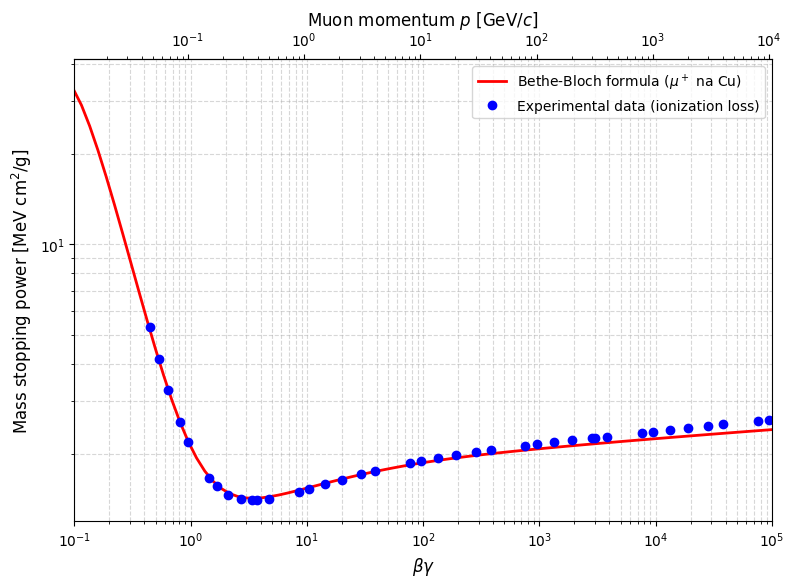
\includegraphics[width=0.6\textwidth]{bethe_bloch.png}
\end{center}
\end{itemize}


\begin{solution}

\end{solution}
%%%%%%%%%%%%%%%%%%%%%%%%%%%%%%%%%%%%%%%%%%%%%%%%%%%%%%%
%%%%%%%%%%%%%%%%%%%%%%%%%%%%%%%%%%%%%%%%%%%%%%%%%%%%%%%
\zadanie[Bragg peak]

Please use the Python function for the Bethe-Bloch formula to calculate energy losses
of 10 GeV muons in copper. Plot the energy loss per step as a function of the step 
number and reproduce the following plot:
\begin{center}
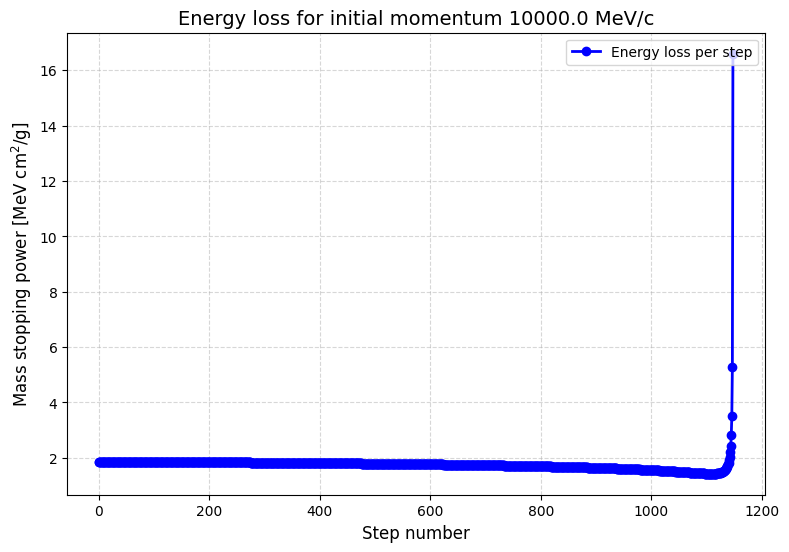
\includegraphics[width=0.6\textwidth]{bragg.png}
\end{center}

What is the name of the curve? 


\begin{solution}

\end{solution}

%%%%%%%%%%%%%%%%%%%%%%%%%%%%%%%%%%%%%%%%%%%%%%%%%%%%%%%
%%%%%%%%%%%%%%%%%%%%%%%%%%%%%%%%%%%%%%%%%%%%%%%%%%%%%%%
\end{document}
